

\section{Compiling JetPack to enable PPS}
\begin{figure}[H]
    \centering
    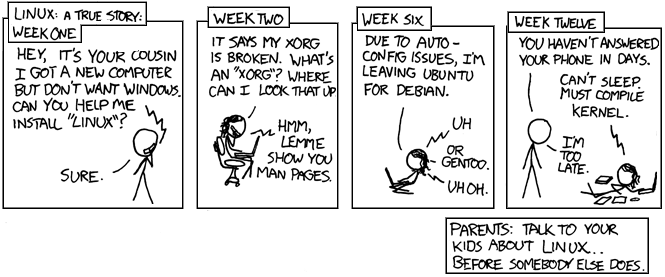
\includegraphics[width=\textwidth]{figures/cautionary.png}
    \caption{Cautionary by XKCD \cite{xkcdCautionary}}
\end{figure}
During the \preproject \gls{pps} interrupts were enabled on the \jx by following a guide from Mateusz Sadowski \cite{sadowskiEnablingPPSJetson2020} \cite[26]{martensPortableSensorRig2022}.
Althogh the guide waw written for Jetson Nano running \gls{jetpack} 4.3, it worked on the \jx running \gls{jetpack} 4.5.1 as well after some minor modifications \cite{sadowskiEnablingPPSJetson2020} \cite[26]{martensPortableSensorRig2022}.
As the \gls{deepstream} \gls{sdk} requires \gls{jetpack} 5.1 or newer, flashing the \jx with the newer version, \gls{jetpack} 5.1.1, while maintaining \gls{pps} interrupts was necessary \cite{nvidiaDeepStreamSDKGet2019}.
The assumption was that this would not be more difficult than doing it with \gls{jetpack} 4.5.1.
This turned out to be wrong.

\subsection{Why it no longer worked}
A significant difference between \gls{jetpack} 4.x.x and \gls{jetpack} 5.x.x is that the former built on the Linux Kernel 4.9 and Ubuntu 18.04
while the latter is built on the Linux Kernel 5.10 and Ubuntu 20.04 \cite{nvidiaJetPackSDK2022}\cite{nvidiaJetPackSDK2023}.
It's hypothesized that the issue is related to this major change, but it is not clear how.
The final solution did not provide much insight either, as it was a combination of several small hacks collected from different sources.

\subsection{The setup}
To flash the \jx it is necessary to have a host computer running Ubuntu 16.04 or 18.04 or 20.04 or 22.04 \cite{nvidiaSDKManager2019}.
During the \preproject I attempted to flash the \jx using a docker image inside \gls{wsl} and communicationg with the \jx over usbipd-win, without success \cite{martensPortableSensorRig2022} \cite{nvidiaSDKManager2019} \cite{dorsselaerUsbipdwin2023}.
Since then some people claim to have acheived this but I was not able to reproduce their result \jx \cite{makinbacon21TUTORIALUsingSdkmanager2022}.
Other posts on the forum appear to confirm my results \cite{2008PleaseProvideMore2022}.
I did however managed to build everything in a docker container on my main computer, copy the files to a local computer and flashing the \jx from there,
but the time saved using a more powerful computer did not outweigh the extra work needed to copy all the files.

Without the possibility to flash from a windows machine, I defaulted to using the same spare laptop as during the \preproject \cite{martensPortableSensorRig2022}.


\subsection{The solution}
Downloading all the necessary files, unpacking them and flashing the \jx took about 2 hours.
With human input requiered every 10-15 minutes on average, it was not really possible to work on finding a solution while doing other work.
The first couple of days were waisted on trying out different things in a very slow tempo.

After having made no real progress and











% \gls{pps} is a high precision signal provided by a device, typically a GPS receiver, that is used to adjust the system clock time with high accuracy. The \gls{pps} signal is often used in combination with \gls{ntpd} to synchronize the system clock with sub-millisecond precision to \gls{utc} \cite{giomettiLinuxPPSWikiLinuxPPS2020}.

% On a \jx it appears necessary to compile the Unix Kernel to enable \gls{pps}.
% How to enable \gls{pps} on the \jx is outlined in the \preproject, but the method presented there no longer works with the newer version of \gls{jetpack}.

\subsection{Preparation}
To flash the \jx it is necessary to have a host computer running Ubuntu 16.04 or 18.04 or 20.04 or 22.04 \cite{nvidiaSDKManager2019}.
Several attempts were made at using the docker image inside \gls{wsl}, communicating with the \jx using usbipd-win, without any success \cite{martensPortableSensorRig2022} \cite{nvidiaSDKManager2019} \cite{dorsselaerUsbipdwin2023}.


